
\subsection{Simple example}

\begin{figure*}
	\centering
	%\subfloat[Topology\label{fig:simple-example:topo}]{%
	%	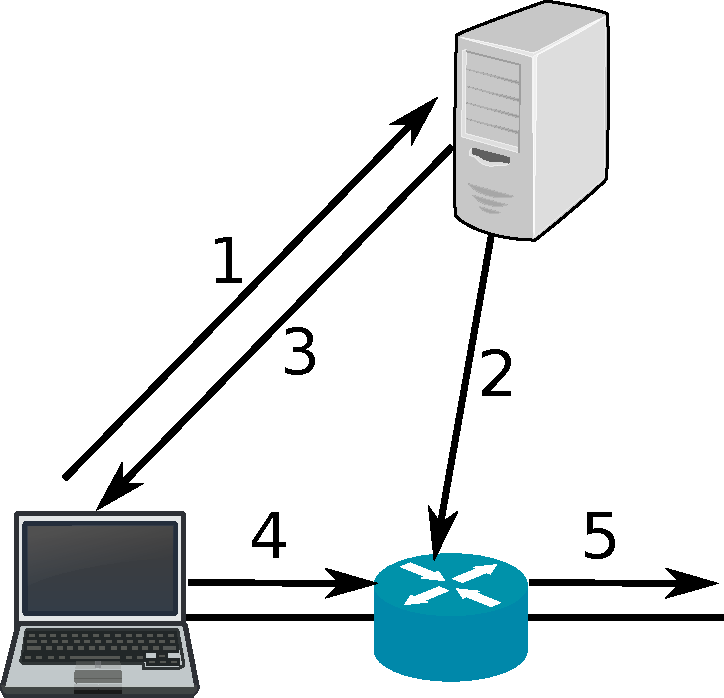
\includegraphics[width=0.3\textwidth]{figs/controller_communication.pdf}
	%}
	\subfloat[Sum of the used network bandwidth\label{fig:simple-example:gamma}]{%
		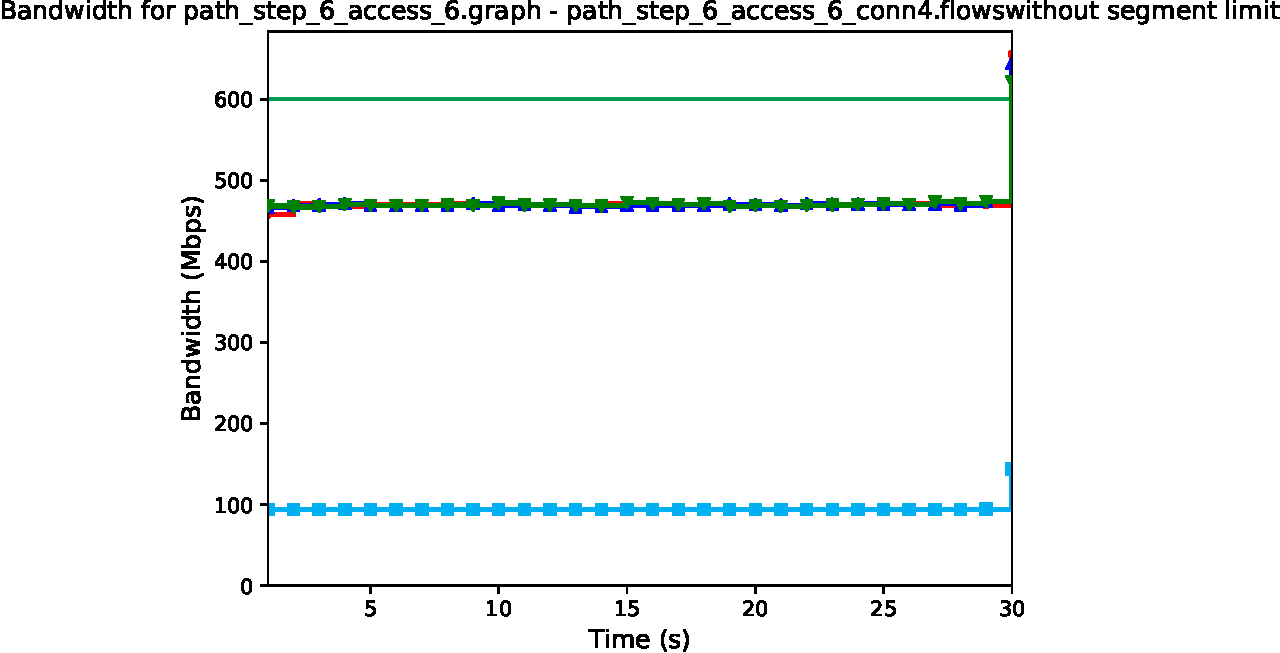
\includegraphics[width=0.6\textwidth]{figs/simple_example_gamma.pdf}
	}
	\caption{Simple example with 6 disjoint paths and 4 clients communicating with 4 servers}
	\label{fig:simple-example}
\end{figure*}

We use the topology shown in Figure \ref{fig:simple-example:topo}.
This simple network only has links with the same bandwidth (100 Mbps) and latency (1ms).
We prevent ECMP from working by setting arbitrary IGP weights on the links.\todo{Test with ECMP enabled}
Each endhost starts 4 connections using iperf3 with the server in front of it the network.
We emulate the network with Mininet\ccite{mininet} on a Linux kernel 5.3
running on machine with 20 CPU and 16 GB of RAM.

Figure \ref{fig:simple-example:gamma} shows the network bandwidth used by all the connections through time.
In theory, this badnwidth could go as high as 600 Mbps according to the Maximum Flow
approximation\ccite{maxflow} since there are six disjoint paths available.
In practice, the total bandwidth is slightly below that number but since this number is above 500Mbps,
we can deduce that all of the six paths are used.
Regular TCP connections, without ECMP, cannot achive more than 100Mbps because they can only use one path.
\todo{Test with ECMP enabled}
We do not see significant changes with different values of \texttt{GAMMA}.
\todo{Discuss with Schapira}

\subsection{Topology Zoo set}

We used 233 topologies from the Topology Zoo\ccite{topologyzoo}.
We modified these topologies to remove part of the graphs that lack link redundancy,\dots trees.
The resulting topologies have only routers with at least two links.
Communication between routers in a tree can only use a single path.
Such trees cannot see any improvement from using Segment Routing.
Moreover, such trees are likely artifacts of the topology collection
because they cannot preserve connectivity even with a single link failure.
Figure \ref{fig:topo:routers} and \ref{fig:topo:links} shows the CDF
of the number of routers and links in the resulting topologies.
Figure \ref{fig:topo:degree} shows the distributions of routers percentage with a given number
of attached links.

\begin{figure*}
	\centering
	\subfloat[Number of routers\label{fig:topo:routers}]{%
		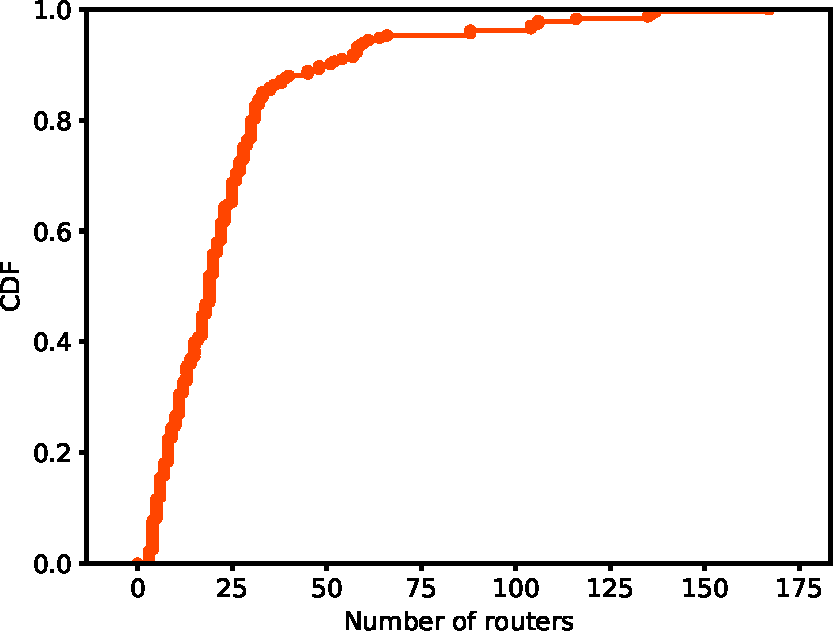
\includegraphics[width=0.3\textwidth]{figs/solver_number_routers_cdfs.pdf}
	}
	\subfloat[Number of links\label{fig:topo:links}]{%
		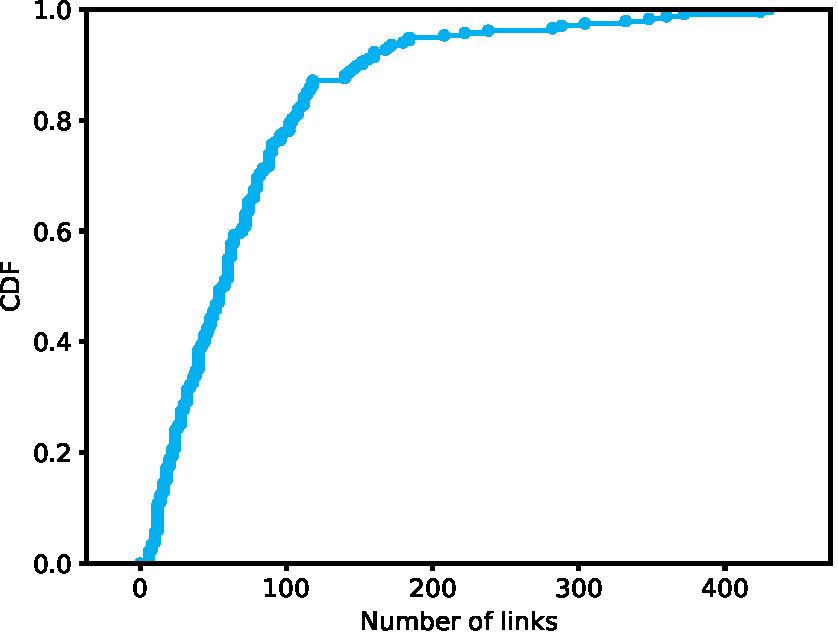
\includegraphics[width=0.3\textwidth]{figs/solver_number_links_cdfs.pdf}
	}
	\subfloat[Out degree of the routers\label{fig:topo:degree}]{%
		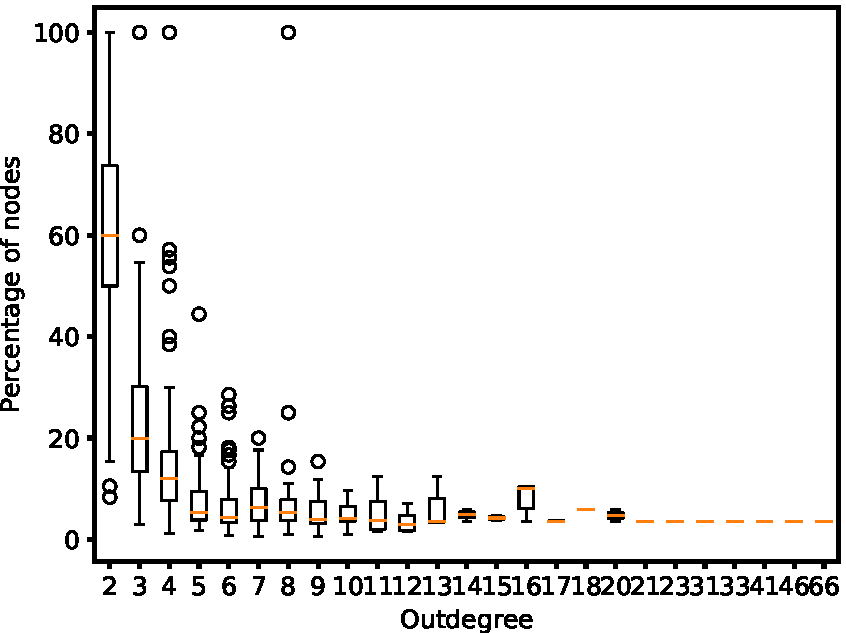
\includegraphics[width=0.303\textwidth]{figs/boxplot_network_outdegree_boxplots.pdf}
	}
	\caption{Features of the evaluation topologies}
	\label{fig:topo}
\end{figure*}

The set of topologies does not include which routers are actually linked to endhosts
and which are core routers. We assume that routers with two links are edge routers
and the others are core routers because they are more connected.

% TODO This implies that a few topologies must be ignored by default

\subsection{Maximum improvement}

This sections evaluation the theoritical improvement of using
multipath transport protocols and Segment Routing on the endhosts
instead of a single path protocol with only shortest paths.

We used a linear programming formulation of the Max Flow problem.
Given a set of paths linking a set of the edge routers, we compute
the maximum amount of traffic that can go through the topology without
exceeding the link capacity.

\begin{equation*}
	\setlength\arraycolsep{0.2pt}
	\begin{smallmatrix}
		\displaystyle maxflow(\P) & & \\
		\displaystyle \max_{f} & \displaystyle \sum_{p \in \P} f_{p} & \\[0.5cm]
		\textrm{s.t.}          & \displaystyle \sum_{p \in \P} \r(l, p) \cdot f_{p} & \displaystyle \leq & \displaystyle \cap(l) & \forall l \in \L
	\end{smallmatrix}
\end{equation*}

$\P$ represents the set of \texttt{sr-paths}, encoded as a list of intermediate routers.
As for IPv6 SR, The real path taken between each intermediate router is the shortest one.
$\r(l, p)$ represents the ratio of flow that goes through a particular link.
This ratio is used to model the ECMP splitting of the traffic.

To model a single-path transport protocol without SR
we insert all the shortest sr-paths between each pair of edge router to $\P$.
We assume that we have a high number of connections for each path
and therefore that hash-based ECMP splits the traffic evenly.
\cite{ecmphashperf} shows that it is not the case in practise.

Multipath transport protocols with SR also uses shortest path routing.
However, they can establish a big number of subflows for each connection
and hope that they will cover all or a portion of the shortest paths.
This hijacks ECMP that sees subflows as indepedent connections.
Flow Bender\ccite{flowbender} and SEMPER\ccite{semper} used this solution to leverage
some of the path diversity of a topology.
We will assume for simplicity that this method works perfectly and that multipath protocols
can always cover all the shortest paths.
We insert a sr-path for each shortest path between each pair of edge routers
instead of giving one sr-path representing all the shortest paths between a given pair. 

Introducing Segment Routing means adding more paths to $\P$.
Note that generating the set of all possible paths is in $\O(|\R|^k)$
with $\R$ being the set of routers and $k$ the maximum number of intermediate nodes.
This is not practicle for big topologies.
Therefore, we reuse the approach of \cite{cg4sr} that iteratively adds relevant paths to the set
until no interesting paths can be added to $\P$.
When it reaches this point, computing the model on this restricted set or on the complete one
gives the same solution.
\todo{Explain how the model is different from infocom, i.e., demands become unbounded or is it too detailed ?}

\textbf{Adding IPv6 SR can significantly improve the maximum throughput.}
Figure \ref{fig:maxflow-theory:tcp} shows the relative maximum flow improvement
of using single path or multiple path with SR.
There is a boxplot for a given percentage of edge router pairs that have heavy hitters
to route \todo{Give the rational behind the choice of the values}.
The number of heavy hitters has influence on the relative improvement.
It is easier to unused alternative paths with fewer heavy hitters.
With 1\% of heavy hitter pairs, for half of the topologies,
we can improve the maximum flow by 71\%.
For 10\% of heavy hitter pairs, we can still improve it by 30\%.
Figure \ref{fig:maxflow-theory:mptcp} shows the improvement with multiple path protocol
without SR.
The improvement is about 5\% lower. This justifies the use of SR even with multipath protocols.

\begin{figure*}
	\centering
	\subfloat[Single path transport protocol\label{fig:maxflow-theory:tcp}]{%
		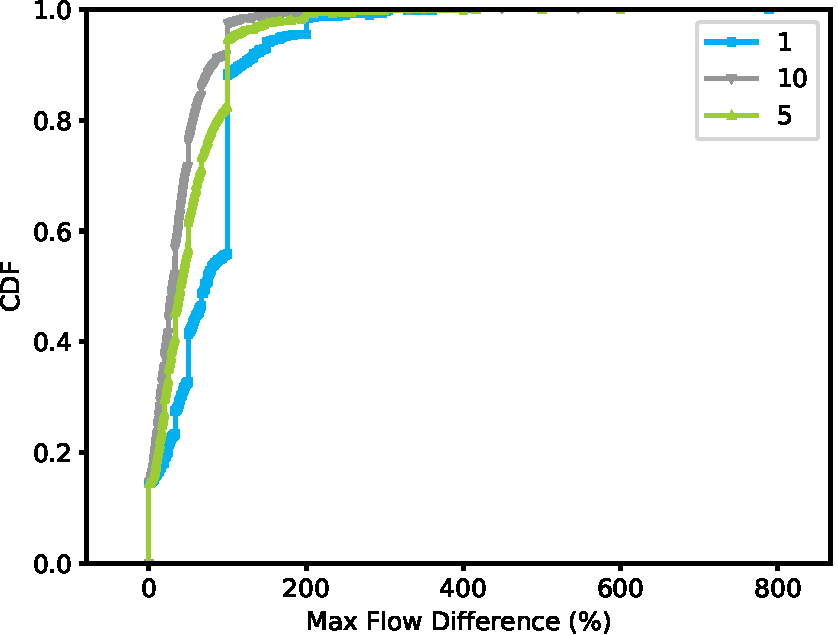
\includegraphics[width=0.4\textwidth]{figs/cdf_maxflow_diff_accesslinks_2_tcp_segs_ecmp_0_0_cdf.pdf}
	}
	\subfloat[Multiple path transport protocol\label{fig:maxflow-theory:mptcp}]{%
		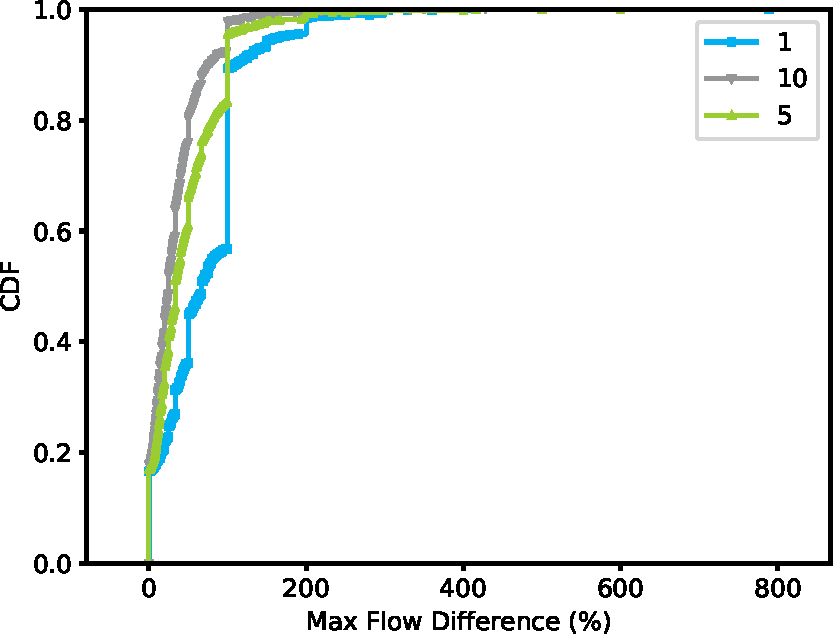
\includegraphics[width=0.4\textwidth]{figs/cdf_maxflow_diff_accesslinks_2_mptcp_segs_ecmp_0_0_cdf.pdf}
	}
	\caption{Relative Maxflow improvement of adding IPv6 SR}
	\label{fig:maxflow-theory}
\end{figure*}

\subsection{Largest set of disjoint paths}

Finding the largest set of disjoint paths between two routers can be done with Edmonds–Karp algorithm \cite{edmondskarp} in O($|\R||\L|^2$).
Even faster strategies can imply applying Dijkstra algorithm iteratively.
Each time that the algorithm finds a path, we remove its links for the next computations.
We stop it when it cannot find another path.
This is solved in O($(|\L|+|\R|)n\log{|\R|}$) with $n$ being the number of iterations of dijkstra algorithm.
O($n$) cannot be bigger than O($|\L|$) because at each iteration, if a path is found, the links if this path will be removed.
In practise, source and destinations are behind routers with exactly two outgoing links.
There will be at most two disjoint paths.
Therefore, applying the Dijkstra algorithm iteratively is faster than using the Edmonds-Karp.

Figure \ref{fig:disjoint:noseglimit} shows a CDF of the mean number of disjoint paths by pair of access router in each topology.
We consider routers with exectly two links as access routers.
This means that there are at least one path between two routers but at most two since there are only two outgoing links.
Edmonds-Karp computes the largest set of disjoint paths that can be reached.
We can reach the same sets for 70\% of topologies by applying iteratively Dijkstra algorithm.

SRv6 is limited in the number of segments that it can apply in a packet.
This limit can be due to hardware limitationsi of IPv6 SR implementations \cite{Tantsura_SID:2017}.
So we need to use algorithms that prevent the number of segments to grow beyond a given limit.
Always finding the largest set of disjoint paths within the limit of segment is exponential and therefore not feasible in practise.
\cite{aubry2015traffic} defines the SPS\todo{Check with Francois for the name} algorithm that computes the shortest path between two routers
under a given limit of segments.
Each time that the algorithm finds a path, they remove all the links for the next computations.
They stop when no more path can be found.
Figure \ref{fig:disjoint:seglimit} shows that the number of disjoint paths increases with the number of authorized segments.
With only one segment, we can only  have one path because only the destination can be encoded in the segment list.
Increasing to 4 segments, (i.e., 3 intermediate routers), signigicantly improves the number of disjoint paths.
We see that increasing the limit beyond this does not improve significantly the number of disjoint paths.

% TODO Figure with iterative dijkstra/warshall as maximum in max seg ?

\begin{figure*}
	\centering
	\subfloat[Without a segment limit\label{fig:disjoint:noseglimit}]{
		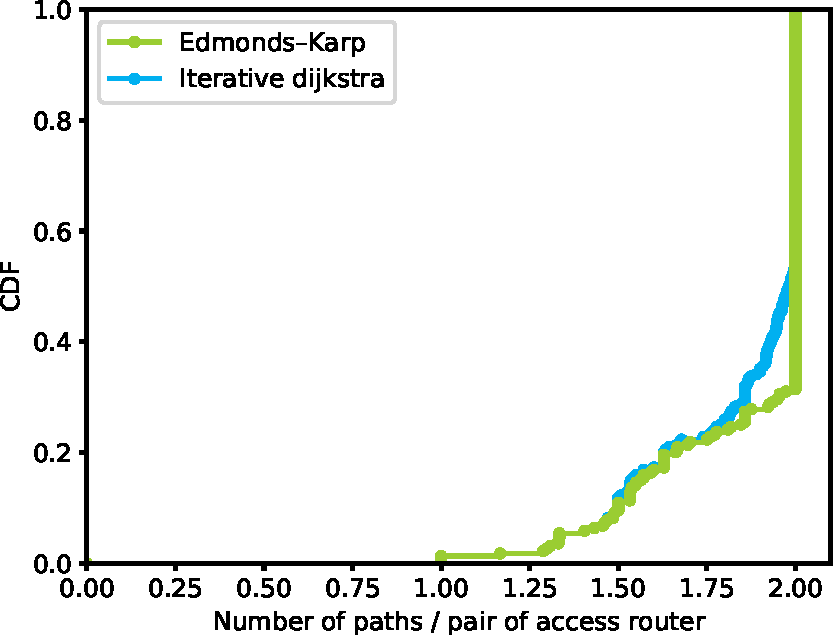
\includegraphics[width=0.4\textwidth]{figs/solver_number_disjoint_paths_cdfs.pdf}
	}
	\subfloat[With a segment limit\label{fig:disjoint:seglimit}]{%
		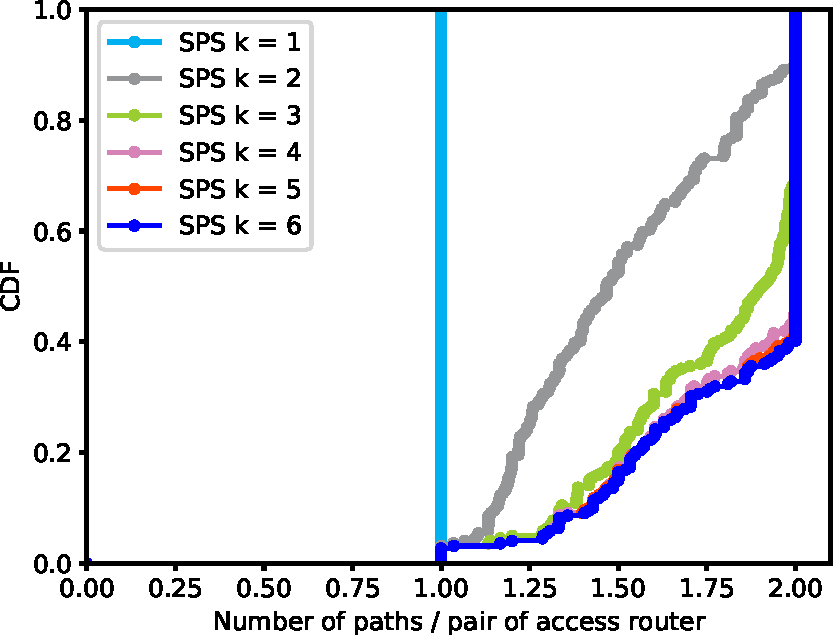
\includegraphics[width=0.4\textwidth]{figs/solver_number_disjoint_paths_max_segs_cdfs.pdf}
	}
	\caption{Number of disjoint paths found by pair of access routers}
	\label{fig:disjoint}
\end{figure*}

